\documentclass[../main.tex]{subfiles}
\graphicspath{{\currfiledir}}
\begin{document}
\chapter{Introduction}
The Maya civilization, which flourished in Mesoamerica from roughly 2000 BCE to 1500 CE 
(\cite[3]{estrada-belli2011}), 
left behind a rich and sophisticated system of hieroglyphic writing. 
These intricate symbols were inscribed on everything from ceramics and sculptures to stairways,
lintels, buildings and monuments (\cite[\ppno~17--27]{thompson1962}), and they recorded everything 
from personal possessions and dedications to religious beliefs, politics and historical events.

In addition to the famous writings on stelas, temples and altars, the Maya also wrote on sheets of 
bark paper (\cite[34\psq]{vonhagen1944}) which were then bundled and 
folded to books (\Cref{fig:introduction-example-dresden-codex} for some sample pages).
These books are usually called \emph{codices}.
\begin{center}
    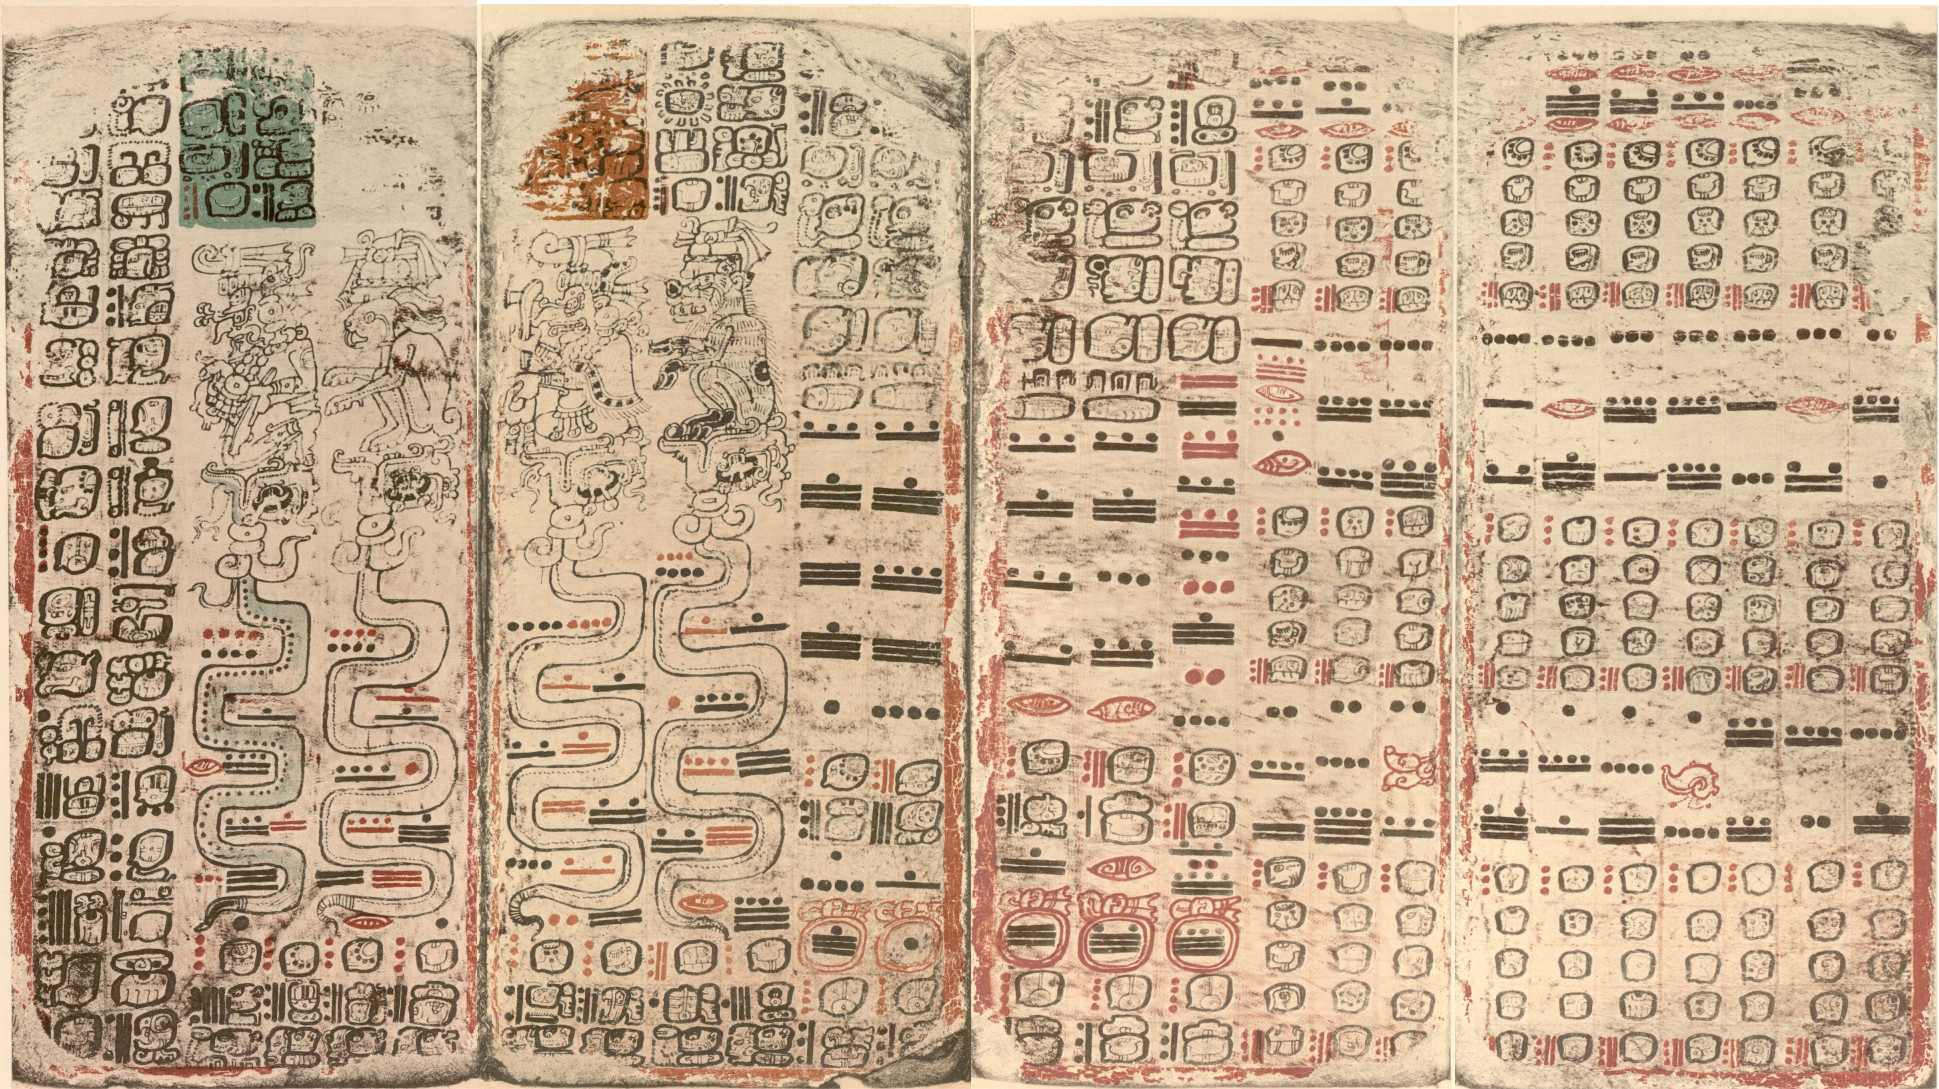
\includegraphics[width=\textwidth,keepaspectratio]{img/example-dresden-codex}
    \captionof{figure}{Sample pages of the \dresdencodex unfolded}
    \label{fig:introduction-example-dresden-codex}
\end{center}
Unfortunately, most of the codices are lost now.
Only four books are known to have survived throughout the time, 
namely the \dresdencodex, the \madridcodex (also called \troanocodex),
the \pariscodex and \mayamexicocodex(also known as \groliercodex).
The codices are named after the location where they have been found or stored.
Hieroglyphs can also be found on incised bones, shells, Jade and Hard stones and on painted or 
carved pottery (\Cref{fig:introduction-panel-with-royal-woman} and
\Cref{fig:introduction-vessel-with-battle-scene}).
% LTeX: enabled=false
\begin{figure}
    \centering
    \subfloat[][]{
        \centering
        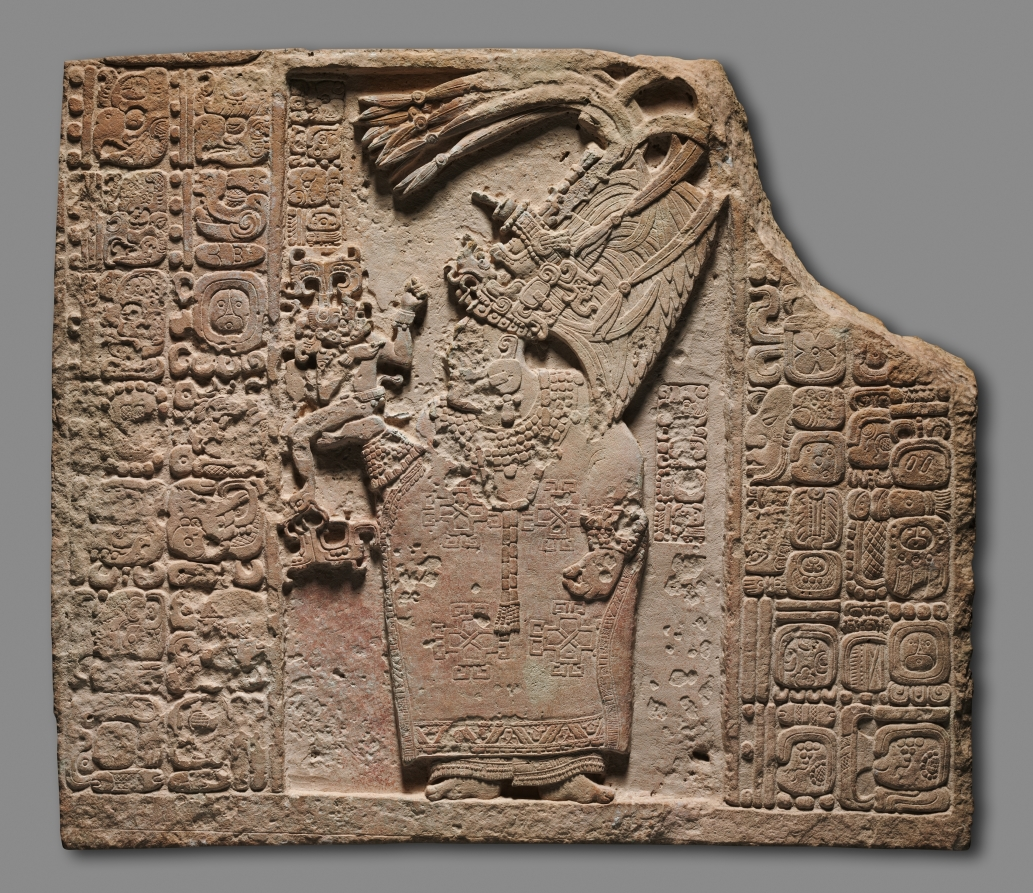
\includegraphics[width=0.47\textwidth]{img/panel-with-royal-woman}
        \label{fig:introduction-panel-with-royal-woman}
    }
    \hfill
    \subfloat[][]{
        \centering
        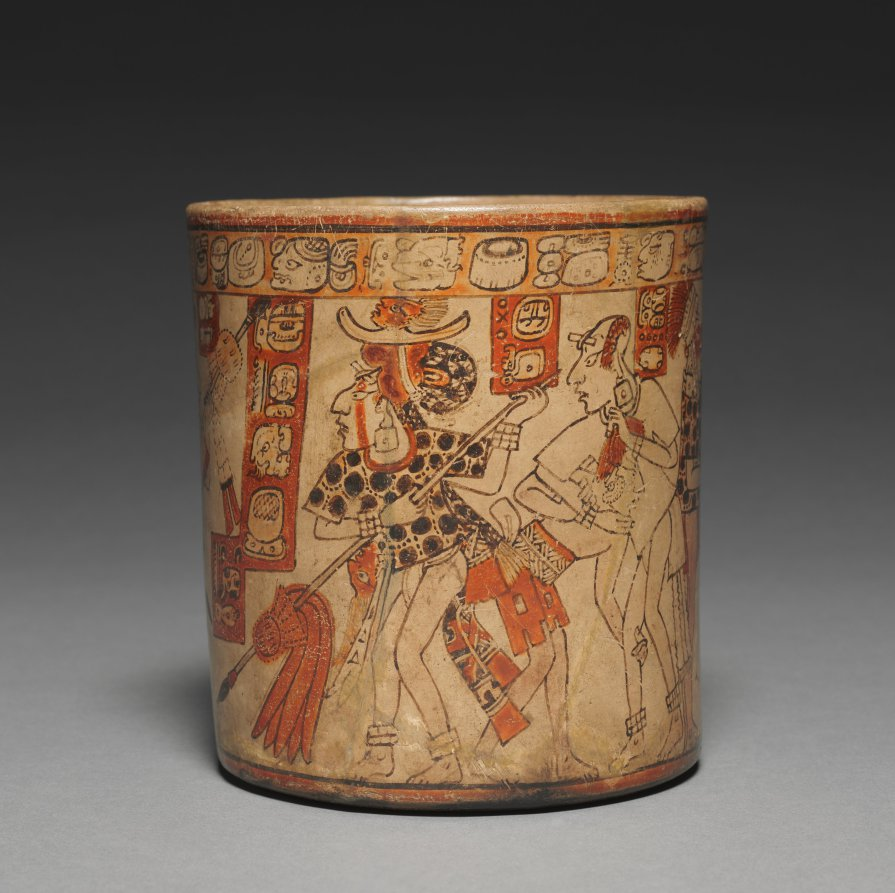
\includegraphics[width=0.47\textwidth]{img/vessel-with-battle-scene}
        \label{fig:introduction-vessel-with-battle-scene}
    }
    \caption[Maya art from the Classic and Late Classic]{Maya art from the Classic and Late Classic.
             \subref{fig:introduction-panel-with-royal-woman} Panel with royal woman, 
             Classic Period, Cleveland Museum of Art, Purchase from the J. H. Wade Fund 1962.32;
             \subref{fig:introduction-vessel-with-battle-scene} Vessel with Battle Scene, 
             Late Classic Period, Cleveland Museum of Art, John L. Severance Fund 2012.32}
\end{figure}
% LTeX: enabled=true

Besides hieroglyphic texts, several manuscripts written in Yucatec Maya using the Latin alphabet 
have been written  during 16th, 17th and 18th century.
% LTeX: enabled=false
\textcquote[68]{brinton1882}{The[se] ``old writings'' \elide were composed by natives 
who had learned to write the Maya in the alphabet adopted by the early missionaries and 
conquerors\elide There were at one time a large number of these records.}
% LTeX: enabled=true
Many Maya villages had such a book.
All books claim to be written by \emph{Chilam Balam} --- a great prophet from the 16th century
who predicted the arrival of the Spaniards in Yucat\'{a}n
(\textcquote[\ppno~186--187]{roys1933}{\elide bearded man would come from the east and 
introduce a new religion}).
Every book is named after the town the manuscript was located in, e.g. 
\emph{The Book of Chilam Balam of Tizimin} originated from \emph{Tizimin} --- a town 
in Yucat\'{a}n
(\Cref{fig:introduction-chilam-balam-of-tizimin-cover-page} shows the title page).
Some other books still exist, many have been lost during the colonial period.
% LTeX: enabled=false
\begin{figure}[ht]
    \centering
    \subfloat[][]{
        \centering
        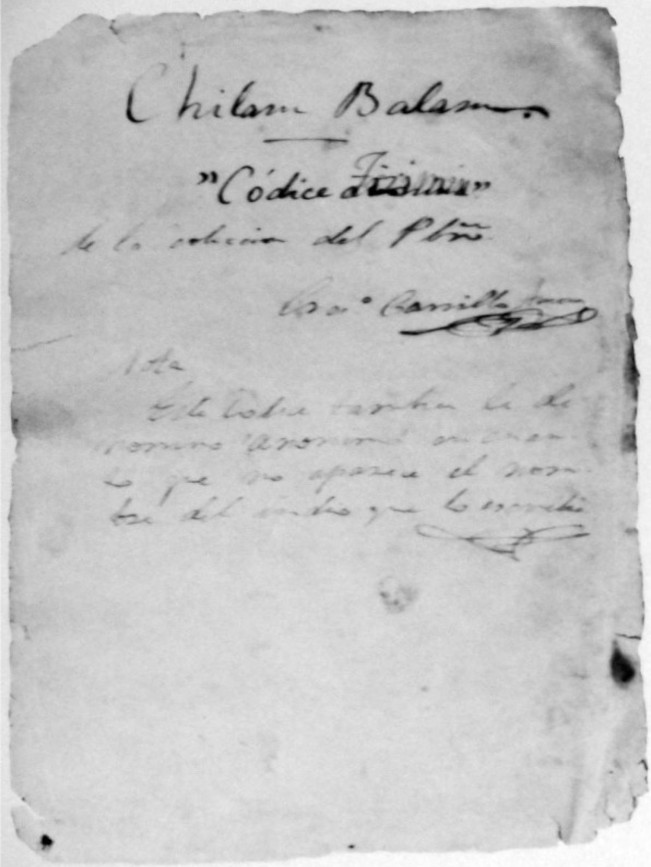
\includegraphics[width=0.47\textwidth]{img/chilam-balam-of-tizimin-cover-page}
        \label{fig:introduction-chilam-balam-of-tizimin-cover-page}
    }
    \hfill
    \subfloat[][]{
        \centering
        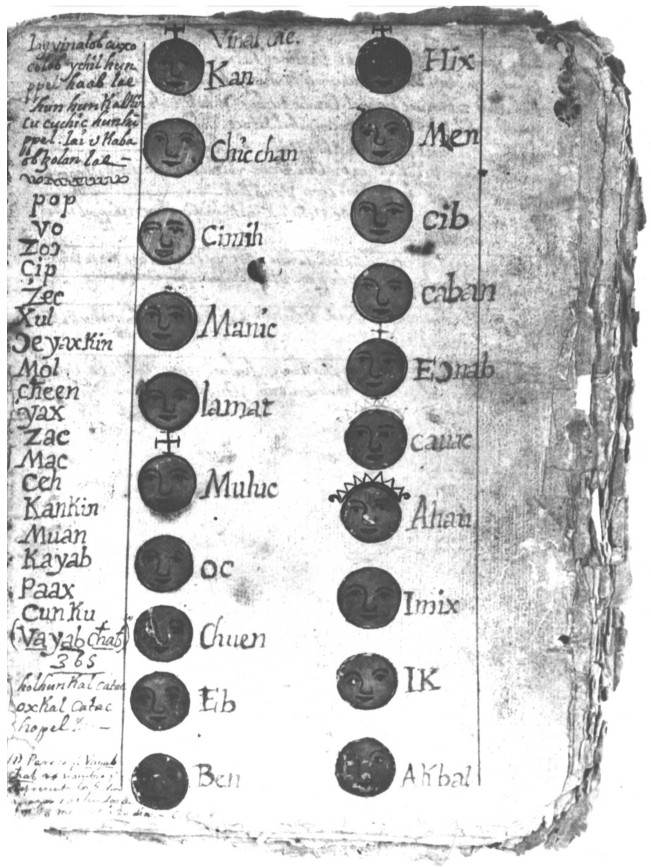
\includegraphics[width=0.47\textwidth]{img/chilam-balam-of-ixil-page-20r}
        \label{fig:introduction-chilam-balam-of-ixil-page-20r}
    }
    \caption[Sample pages of the books of \emph{Chilam Balam}]{Sample pages of the books of 
             \emph{Chilam Balam}.
             \subref{fig:introduction-chilam-balam-of-tizimin-cover-page} Cover of the 
             \emph{Book of Chilam Balam of Tizimin} (\emph{Chilam Balam ``C\'odice Tizimin''});
             \subref{fig:introduction-chilam-balam-of-ixil-page-20r} Page 20r of 
             \emph{Book of Chilam Balam of Ixil}. It shows the \haab months and \tzolkin days.}
\end{figure}
% LTeX: enabled=true
These books also play an important role during the process of hieroglyphic decipherment as they 
contain vital information about historical events, calendrical information, ritual and 
medical descriptions and many more aspects which help to analyze the great writings of the 
Maya (\cite[3\psq]{roys1933}).
For instance, some pages of these books for instance, shows some 
calendrical information from the \tzolkin and \haab calendars 
(\Cref{fig:introduction-chilam-balam-of-ixil-page-20r}).

\section{Early attempts in deciphering the Maya hieroglyphs}
For centuries, the hieroglyphic writings remained largely mysterious, as the Maya script was 
undeciphered and the language spoken by the ancient Maya was largely unknown.
It was not until the late 19th and early 20th centuries that scholars made significant progress 
in deciphering a large range of Maya hieroglyphs and understanding the grammar and syntax of 
the Maya language. 

One breakthrough in the decipherment of Maya hieroglyphs came in the 1960s, 
when Yuri Knorosov (\cite{knorozov1967}) demonstrated that the script was a fully developed 
system of writing, with a phonetic component as well as a logographic component. 
Although his work is often cited in many sources, many advances before him and after his efforts
were necessary to unlock the mysteries of the Maya hieroglyphs.
Nevertheless, his discovery allowed scholars to begin analyzing Maya texts in a more systematic 
way and paved the way for further research into the language and culture of the ancient Maya.

The decipherment was only possible thanks to the hard work of dedicated scholars, epigraphs, 
linguists and archaeologists. 
These individuals dedicated their lives to studying the Maya civilization and its written 
language, and their efforts have helped to shed light on this ancient culture and its way of life. 

Today, the decipherment of Maya hieroglyphs continues to be an active field of study, 
and new insights into the language and culture of the ancient Maya are being discovered 
all the time (\cite{zender2017}). 
The decipherment of Maya hieroglyphs has not only shed light on the rich history and culture of 
the Maya, but has also helped to deepen our understanding of the development of writing and 
language in general.
There are still many questions and not all signs can be read, and even of those which can be read
many signs are still not fully understood.
Yet, it is fascinating that it was possible to decipher most parts
and the nature of the script up to a degree so that scholars are able to read the writings and 
understand the texts on the monuments and objects.

This work will explore the fascinating history of the decipherment of Maya hieroglyphs, 
from the early attempts to understand these symbols to the modern techniques used to unlock 
their secrets. Along the way, one will learn about the key figures who made significant 
contributions to this field and the impact their work has had on the understanding of the 
Maya civilization.
As the decipherment is an ongoing process, this work ``The History of Decipherment'' is not a 
finalized document.
It will evolve through time and each release will tell more and more 
about the history of decipherment of Maya hieroglyphs.

\section{Outlook}
This work would like to take the reader on the journey on how the Maya hieroglyphs actually 
have been deciphered.
It wants to address questions like `How did scholars deduce the meaning of sign X?',
`What are the methods and the science to actually approach an almost unknown script' and many more.
The general idea is, to lay out the historical process of decipherment of the Maya script.

The journey is about to start in the past around 1830
followed by the discovery of an old script presumably written by the Spanish bishop Diego de Landa 
in the 16th century.
Then, the focus will move on to discoveries made in the 19th and 20th century up until today.
As the book progresses, more and more insights in the Maya script will be revealed.

The upcoming chapters are organized in a chronological way to explain the progress and the 
discoveries made by so many scholars.
Even though, the book tries to tell the story of decipherment chronologically, sometimes
the narrative will jump back and forth in time to ease the understanding of 
the decipherment process.
Every scientific work, its discovery and additional information will be cited along the way and 
will be provided as a reference to the reader.
However, not every decipherment can be described in detail, but the provided sources should help 
the reader to reach out to additional literature.
This work will provide as many details as possible to make sure the readers understands the 
reasoning behind the decipherment, so that the progress of decipherment is 
conclusive and consistent.

\end{document}
